\chapter[Equ. 2nd degré]{Équations du second degré}
\thispagestyle{fancy}

\section{Résolution d'une équation du second degré}

\subsection{Résoudre une équation à l'aide du discriminant}

    \begin{definition}
        Une \grasInDef{équation du second degré} est une équation de la forme $ax^2+bx+c=0$ où $a$, $b$ et $c$ sont des réels avec $a\neq 0$.\\
        Une solution de cette équation s'appelle une \grasInDef{racine} du trinôme $ax^2+bx+c$.
    \end{definition}
    
    \begin{exemple}
        L'équation $3x^2-6x-2=0$ est une équation du second degré.
    \end{exemple}
    
    % \begin{remarque}
    %     Résoudre l'équation $3x^2-6x-2=0$ ou trouver les racines du trinôme $3x^2-6x-2$ sont deux énoncés identiques.
    % \end{remarque}
        
    \begin{definition}
        On appelle \grasInDef{discriminant} du trinôme $ax^2+bx+c$, le nombre réel, noté $\Delta$, égal à $b^2-4ac$.
        $$\Delta = b^2-4ac$$
    \end{definition}
        
    \begin{propriete}
        Soit $\Delta$ le discriminant du trinôme $ax^2+bx+c$.\\
        \begin{itemDef}
            \item Si $\Delta < 0$ : L'équation $ax^2+bx+c=0$ n'a pas de solution réelle.
            \item Si $\Delta = 0$ : L'équation $ax^2+bx+c=0$ a une unique solution : $x_0= \dfrac{-b}{2a}$.
            \item Si $\Delta > 0$ : L'équation $ax^2+bx+c=0$ a deux solutions distinctes :\\
            \hspace*{3cm} $x_1= \dfrac{-b-\sqrt{\Delta}}{2a}$ \hspace*{0.5cm} et \hspace*{0.5cm} $x_2= \dfrac{-b+\sqrt{\Delta}}{2a}$
        \end{itemDef}         
    \end{propriete}
        
        
    \begin{methodeTitre}{Résoudre une équation du second degré}
        \grasInMet{Enoncé :} Résoudre les équations suivantes : 
        \begin{enumerate}
            \item $2x^2-x-6=0$
            \item $2x^2-3x+\dfrac{9}{8}=0$.
            \item $x^2+3x+10=0$
        \end{enumerate}
        \grasInMet{Réponse :}\\
        \begin{enumerate}
            \item Calculons le discriminant de l'équation $2x^2-x-6=0$ :\\
            $a = 2$, $b = -1$ et $c = -6$ donc $\Delta = b^2-4ac = (-1)^2 - 4 \times 2 \times (-6) = 49$.\\
            Comme $\Delta > 0$, l'équation possède deux solutions distinctes :\\
            \hspace*{2cm} $x_1= \dfrac{-b-\sqrt{\Delta}}{2a}=\dfrac{-(-1)-\sqrt{49}}{2\times2}=-\dfrac{3}{2}$\\
            \hspace*{2cm} $x_2= \dfrac{-b+\sqrt{\Delta}}{2a}=\dfrac{-(-1)+\sqrt{49}}{2\times2}=2$
            \item Calculons le discriminant de l'équation $2x^2-3x+\dfrac{9}{8}=0$ :\\
            $a = 2$, $b = -3$ et $c = \dfrac{9}{8}$ donc $\Delta = b^2-4ac = (-3)^2 - 4 \times 2 \times \dfrac{9}{8} = 0$.\\
            Comme $\Delta = 0$, l'équation possède une solution unique :\\
            \hspace*{2cm} $x_0= -\dfrac{b}{2a}=-\dfrac{-3}{2\times2}=\dfrac{3}{4}$\\
            \item Calculons le discriminant de l'équation $x^2+3x+10=0$ :\\
            $a = 1$, $b = 3$ et $c = 10$ donc $\Delta = b^2-4ac = 3^2 - 4 \times 1 \times 10 = -31$.\\
            Comme $\Delta < 0$, l'équation ne possède pas de solution réelle.
        \end{enumerate}
    \end{methodeTitre}
    
\subsection{Résoudre une équation à l'aide de la somme et du produit des racines}
    
    \begin{propriete}
        La somme $S$ et le produit $P$ des racines d'un polynôme du second degré de la forme $ax^2+bx+c$ sont donnés par : $S=- \dfrac{b}{a}$  et $P= \dfrac{c}{a}$. 
    \end{propriete}
    
    \begin{demonstration}
        \begin{itemDem}
            \item $S=x_1+x_2=\dfrac{-b-\sqrt{\Delta}}{2a}+\dfrac{-b+\sqrt{\Delta}}{2a}=\dfrac{-b-\sqrt{\Delta}-b+\sqrt{\Delta}}{2a}=\dfrac{-2b}{2a}=- \dfrac{b}{a}$
            \item $P=x_1\times x_2=\dfrac{-b-\sqrt{\Delta}}{2a}\times \dfrac{-b+\sqrt{\Delta}}{2a}=\dfrac{(-b-\sqrt{\Delta})\times(-b+\sqrt{\Delta})}{4a^2}=\dfrac{b^2-\Delta}{4a^2}=\dfrac{b^2-b^2+4ac}{4a^2}=\dfrac{c}{a}$
        \end{itemDem}
    \end{demonstration}
    
    \begin{methodeTitre}{utiliser somme et produit pour trouver les 2 racines}
        \grasInMet{Enoncé :}\\
        Trouver les 2 racines du polynôme suivant : $2x^2+3x-5$\\
        \grasInMet{Réponse :}\\
        On a une solution évidente ($x_1=1$). Or la somme des 2 racines vaut $S=- \dfrac{b}{a}=-\dfrac{3}{2}$. Donc:\\
        $x_1+x_2=-\dfrac{3}{2} \iff 1+x_2=-\dfrac{3}{2} \iff x_2=-\dfrac{3}{2}-1=-\dfrac{5}{2}$
    \end{methodeTitre}
        
    
\section{Factorisation d'un trinôme}

    \begin{propriete}
        Soit $f$ une fonction polynôme de degré 2 définie sur \R  par $f(x)=ax^2+bx+c$.
        \begin{itemDef}
            \item Si $\Delta = 0$ : Pour tout réel $x$, on a : $f(x)=a(x-x_0 )^2$ avec $x_0$ racine unique du trinôme.
            \item Si $\Delta > 0$ : Pour tout réel $x$, on a : $f(x)=a(x-x_1 )(x-x_2 )$ avec $x_1$ et $x_2$ les 2 racines du trinôme..
        \end{itemDef}
    \end{propriete}
    
    \begin{remarque}
        Si $\Delta < 0$, il n'existe pas de forme factorisée de $f$.
    \end{remarque}
    
    \begin{methodeTitre}{Factoriser un trinôme}
        \grasInMet{Enoncé :} Factoriser les trinômes suivants
        \begin{enumerate}
            \item $4x^2+19x-5$
            \item $9x^2-6x+1$.
        \end{enumerate}
        \grasInMet{Réponse :}
        \begin{enumerate}
            \item On cherche les racines du trinôme $4x^2+19x-5$:\\
            Calcul du discriminant : $\Delta = 19^2 - 4 \times 4 \times (-5) = 441$\\
            Les racines sont : $x_1= \dfrac{-19-\sqrt{441}}{2\times4} = \mVert{-5}$  et  $x_2= \dfrac{-19+\sqrt{441}}{2\times4}  = \mVert{\dfrac{1}{4}}$\\
            On a donc :\\
            $\mRouge{4}x^2+19x-5=\mRouge{4}\left(x-(\mVert{-5})\right)\left(x-\mVert{\dfrac{1}{4}}\right)=(x+5)(4x-1)$
            \item On cherche les racines du trinôme $9x^2-6x+1$ :\\
            Calcul du discriminant : $\Delta = (-6)^2 - 4 \times 9 \times 1 = 0$\\
            La racine (double) est : $x_0=- \dfrac{-6}{2\times 9} = \mVert{\dfrac{1}{3}}$\\   
            On a donc :\\
            $\mRouge{9}x^2-6x+1=\mRouge{9} \left( x-\mVert{\dfrac{1}{3}} \right) ^2$
        \end{enumerate}
    \end{methodeTitre}
    
    \begin{remarque}
        On peut vérifier le résultat à l'aide de la calculatrice. En traçant la courbe représentative de la fonction, on peut vérifier les racines à l'aide des points d'intersection de la courbe et de l'axe des abscisses. Ainsi en traçant les courbes précédentes, nous obtenons les courbes suivantes:
        %\begin{multicols}{2}
            \includegraphics[scale=0.85]{01-03-01}
            \includegraphics[scale=0.85]{01-03-02}
        %\end{multicols}
    \end{remarque}
    
\section{signe d'un trinôme}

    \begin{remarqueTitre}{préliminaire}
        Pour une fonction polynôme de degré 2 définie par $f(x)=ax^2+bx+c$ :
        \begin{itemRem}
            \item si $a > 0$, sa représentation graphique est une parabole tournée vers le haut.
            \item si $a < 0$, sa représentation graphique est une parabole tournée vers le bas
        \end{itemRem}
    \end{remarqueTitre}
    
    \begin{propriete}
        Soit $f$ une fonction polynôme de degré 2 définie sur \R par $f(x)=ax^2+bx+c$:
        \begin{itemDef}
            \item si $\Delta < 0$:\\
            %\begin{minipage}[b]{0.5\linewidth}
                \begin{tikzpicture}
                   \tkzTabInit{$x$ / 1 , $f(x)$ / 1}{$-\infty$, $+\infty$}
                   \tkzTabLine{, \text{signe de } a, }
                \end{tikzpicture}
            %\end{minipage}
            %\begin{minipage}[b]{0.48\linewidth}
                \includegraphics[scale=0.85]{01-03-03}      
            %\end{minipage}
            \item si $\Delta = 0$:\\
            %\begin{minipage}[b]{0.6\linewidth}
                \begin{tikzpicture}
                   \tkzTabInit{$x$ / 1 , $f(x)$ / 1}{$-\infty$, $x_0$, $+\infty$}
                   \tkzTabLine{, \text{signe de } a, z, \text{signe de } a, }
                \end{tikzpicture}
            %\end{minipage}
            %\begin{minipage}[b]{0.38\linewidth}
                \includegraphics[scale=0.85]{01-03-04}      
            %\end{minipage}
            \item si $\Delta > 0$:\\
            %\begin{minipage}[b]{0.67\linewidth}
                \begin{tikzpicture}
                   \tkzTabInit[lgt = 1.2, espcl = 2.8, deltacl = 0.5]{$x$ / 1 , $f(x)$ / 1}{$-\infty$, $x_1$,$x_2$, $+\infty$}
                   \tkzTabLine{, \text{signe de } a, z, \text{signe de } -a,z, \text{signe de } a,}
                \end{tikzpicture}
            %\end{minipage}
            %\begin{minipage}[b]{0.31\linewidth}
                \includegraphics[scale=0.85]{01-03-05}      
            %\end{minipage}
        \end{itemDef}
    \end{propriete}
    
    \begin{methodeTitre}{Résoudre une inéquation du second degré}
        \grasInMet{Enoncé :} Résoudre l'inéquation : $x^2+3x-5<-x+2$\\
        \ \\
        \grasInMet{Réponse :}\\
            \emph{On commence par rassembler tous les termes dans le membre de gauche afin de pouvoir étudier les signes des trinômes.}\\
            $x^2+3x-5<-x+2$ équivaut à $x^2+4x-7<0$.\\
            Le discriminant de $x^2+4x-7$ est $\Delta = 16 - 4 \times 1 \times (-7) = 44$ et ses racines sont :\\
            $x_1= \dfrac{-4-\sqrt{44}}{2\times1}=-2-\sqrt{11}$ et $x_2= \dfrac{-4+\sqrt{44}}{2\times1}=-2+\sqrt{11}$\\
            On obtient le tableau de signes :\\
            \begin{tikzpicture}
               \tkzTabInit{$x$ / 1 , $f(x)$ / 1}{$-\infty$,$-2-\sqrt{11}$, $-2+\sqrt{11}$, $+\infty$}
               \tkzTabLine{, +, z,- , z, +, }
            \end{tikzpicture}\\
            L'ensemble des solutions de l'inéquation $x^2+3x-5<-x+2$  est donc $\intervOO{-2-\sqrt{11}}{-2+\sqrt{11}}$.
    \end{methodeTitre}
    
    \begin{remarque}
        Comme précédement, on peut vérifier le résultat à l'aide de la calculatrice.\\
            \begin{center}
                \includegraphics[scale=0.85]{01-03-06}
            \end{center}
    \end{remarque}


